\scanpage{121}
% archive sheet number: 120

6) Supposons maintenant que $C$ soit une catégorie \deleted{additive}\inserted{abélienne} $k$-linéaire ($k$ un corps) munie d'un foncteur fidèle exact $F:C\handwritten{\to}\mathrm{Modf}(k)$, de sorte que $C$ s'identifie à la catégorie des représentations \deleted{d'un}\inserted{(continues)} finies d'une algèbre profinie $U$ sur $k$\inserted{(associative, unitaire)}, ou des comodules sur le dual\inserted{topologique} $A$ de $k$, qui est une coalgèbre (associative, unitaire). Alors la donnée d'un foncteur $\otimes$\inserted{bilinaire} compatible avec $F$ (i.e. pour lequel \deleted{c'est} on a \uline{égalité} $F(X\otimes Y)=F(X)\otimes F(Y)$) \uline{équivaut} à la donnée d'un morphisme diagonal $U\handwritten{\to}U\overset{\handwritten{\scriptscriptstyle\wedge}}{\otimes}_k U$, ou encore d'une loi de multiplication sur $A$. Une donnée supplémentaire (au sens de 4)) a) \deleted{b)}\inserted{\handwritten{b)}} ou c) \uline{compatible} avec $F$, $c=\mathrm{id}$ est alors uniquement déterminée, si elle existe.\inserted{\handwritten{\deleted{\unsure{pour b)} \unsure{il} \illegible{4} \unsure{que soit une} $\unsure{\epsilon|\varepsilon}:U\to k$ (\unsure{hom. de $k$-alg}) i.e. $\epsilon\in A$ \unsure{et que ce soit}}}} Elle existe sss $A$ est associative, resp. unitaire resp. commutative. Quand ces conditions sont satisfaites simultanément, on a donc un schéma en \deleted{groupes}\inserted{\handwritten{monoïdes}} affine sur $k$, qui permet de réconstituer la situation. - Si on a de même $\mathbb{C}',F'$ sur le même $k$, \deleted{avec un $\otimes$,} alors les foncteurs $G:C\handwritten{\to} C'$ compatibles avec $F,F'$ correspondent exactement aux hom. de $k$-algèbre top $U'\handwritten{\to}U$, ou de $k$-coalgèbres $A\handwritten{\to}A'$. Si $\mathbb{C}$ et $C'$ sont munis de structures bilinéaires $\otimes\handwritten{\unsure{,|/}}\otimes$, alors le foncteur $G$ est un $\otimes$-foncteur avec un isomorphisme $c$ transformé par $F'$ en $\mathrm{id}$ (ce qui suffit à \deleted{le} caractériser\inserted{\handwritten{$c$}} alors) sss $U'\handwritten{\to}U$ est compatible avec les diagonales i.e. $A\handwritten{\to}A'$ est compatible avec les multiplications. Les éventuelles structures supplémentaires a) \deleted{b)} ou c) sont respectées automatiquement,\inserted{\handwritten{pour b) il faut imposer compatibilité aux \unsure{augm.|augm} de $U$ resp. aux unités de $A,A'$}}

\margin{généraliser au moins partiellement au cas d'un $k$ qui n'est pas un corps}

\margin{\figure{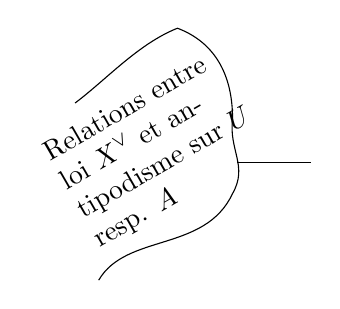
\begin{tikzpicture}[baseline]
\draw (0,0) .. controls (.35,.6) and (1.35,.35) .. (1.7,1.1) .. controls (1.9,1.45) and (1.65,1.65) .. (1.7,2.05) .. controls (1.7,2.7) and (1.4,3.05) .. (1,3.2) .. controls (.5,3) and (.1,2.55) .. (-.3,2.25);
\draw (1.76,1.5)--(2.7,1.5);
\node[rotate=30,align=left,text width=2.65cm] at (.8,1.7) {\handwritten{Relations entre\\loi $X^\vee$ et antipodisme sur $U$\\resp. $A$}};
\end{tikzpicture}}}

\figure{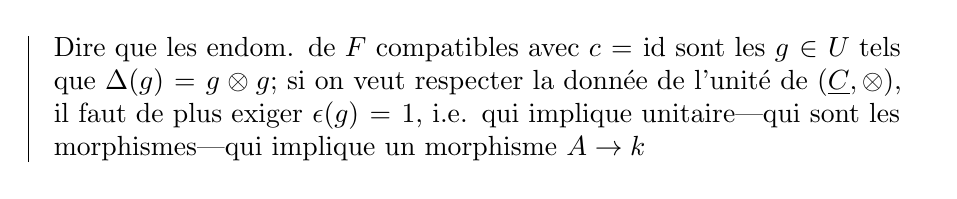
\begin{tikzpicture}[baseline]
\draw (0,0)--(0,1.6);
\node[anchor=west,align=left,text width=11cm] at (.2,.8) {\handwritten{Dire que les endom. de $F$ compatibles avec $c=\mathrm{id}$ sont les $g\in U$ tels que $\Delta(g)=g\otimes g$; si on veut respecter la donnée de l'unité de $(\underline{C},\otimes)$, il faut de plus exiger $\epsilon(g)=1$, i.e. \unsure{qui implique unitaire|qui sont les morphismes|qui implique un morphisme} $A\to k$}};
\end{tikzpicture}}

7) Un exemple. On prend pour $C$ la catégorie des modules gradué\unsure{ss|s} sur un anneau commutatif $\mathbb{k}$, avec le produit tensoriel gradué ordinaire et pour unité le module $\mathbb{k}_s$ gradué par le degré zéro, donnée\deleted{\unsure{di}} de $u$ et $v$ comme d'habitude, ainsi que $\handwritten{\phi}$ (associativité) et $\handwritten{\unsure{\mu|\psi}}$ (commutativité). Tous les axiomes du nº1 sont vérifiés, et le foncteur oubli (avec $c=\mathrm{id}$) estnun $\otimes$-foncteur respectant toutes les données a)b)c). Donc si $k$ est
